% ED-09 -- The bilayer dipolar-exciton interaction is completely monotone
% English translation of papers/discovery_journal_2026/chapters/c09.tex
% Sources: TOP20.json pick 9; papers/ar_dipolar_exciton/{AUDIT.md,REVISION.md,publication_meta.json,gen_numbers.tex,
%          data/lattice_gaps.jsonl}
% Figure: code/fig09.py -> figures/c09_dipoles.{pdf,png}
\chapter[Excitons in triangles]{Electron--hole pairs that arrange themselves in triangles, on paper}
\reference{Preprint of 25 October 2026.\\ doi:10.5281/\\zenodo.23646103}

\section*{The idea in one picture}

\begin{analogie}
A guarantee already exists: ``any recipe whose ingredients meet such-and-such specification gives a successful
dish.'' We do not redo the guarantee; we take a new ingredient, check point by point that it meets the
specification, and the guarantee then applies to it. Here, the guarantee is the triangular-lattice theorem from the
openai/math repository, the specification is the property called ``completely monotone'', and the new ingredient is
the repulsion between two excitons in a stack of two atomic layers.

\emph{Where the picture stops being accurate:} the guarantee itself has not been peer reviewed, and it concerns
classical particles standing still at absolute zero; real excitons, at these densities, form a quantum gas.
\end{analogie}

\section*{What was done}

An exciton is a bound pair made of an electron and a ``hole'' (an absence of an electron, with positive charge).
When the electron lives in one layer and the hole in the neighbouring layer, at distance $d$, the pair becomes a
small vertical dipole. Two such dipoles, at distance $r$ in the plane, repel each other: the two electrons repel,
so do the two holes (two $1/r$ terms), and each electron attracts the other's hole across the gap (two
$1/\sqrt{r^2+d^2}$ terms). Net result:
\[
V(r)=2\Bigl(\frac1r-\frac1{\sqrt{r^2+d^2}}\Bigr).
\]
The article proves in Lean that this repulsion, seen as a function of the squared distance $t=r^2$, has the
property required by the upstream theorem: it is positive, it decreases, its slope flattens out, and so on with
signs that alternate at every order of differentiation. From this it deduces that the triangular lattice has the
lowest energy among all configurations, \emph{at all densities}, and that this energy is finite (otherwise the
inequality would say nothing useful).

\begin{encadre}
\textbf{To do with a pencil.} Take $d=1$.
\begin{itemize}
\item At distance $r=1$: $V=2(1-1/\sqrt2)=2-\sqrt2\approx0.586$.
\item At distance $r=10$: $V=2(0.1-1/\sqrt{101})\approx2(0.1-0.099504)\approx0.000993$, almost exactly
  $d^2/r^3=0.001$. From far away, the pair behaves like a dipole (figure~\ref{fig:c09}, left).
\item The signs, at $t=1$ with $d^2=3$: $g(t)=2(t^{-1/2}-(t+3)^{-1/2})$ equals $2(1-\tfrac12)=1>0$; its derivative
  equals $-(1-\tfrac18)=-\tfrac78<0$; its second derivative equals $\tfrac32(1-\tfrac1{32})=\tfrac{93}{64}>0$. The
  signs alternate, as the specification demands.
\item Counter-test: with a negative shift, $t^{-1/2}-(t-c)^{-1/2}$ ($c>0$) is \emph{negative}; the property
  fails, and Lean proves that too.
\end{itemize}
\end{encadre}

\begin{figure}[htbp]
\centering
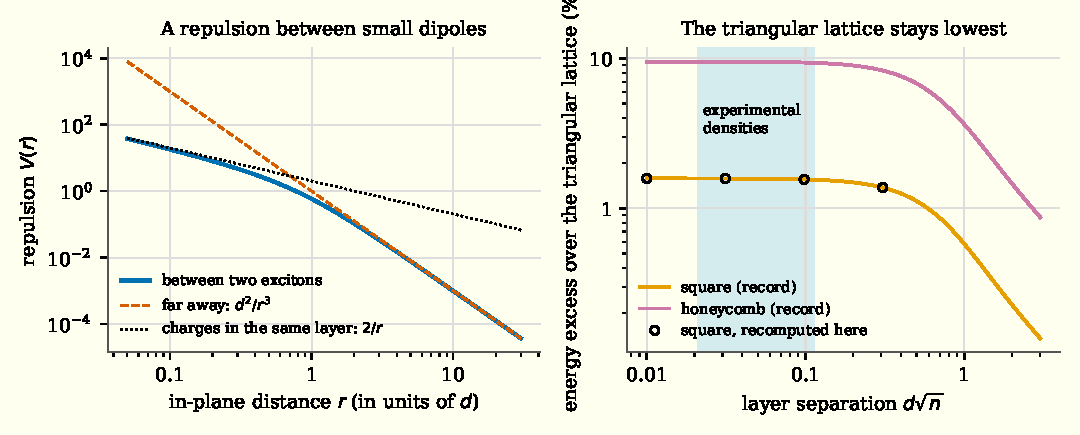
\includegraphics[width=\linewidth]{figures/c09_dipoles}
\caption{The repulsion between dipoles (left); energy excess of the square and honeycomb lattices (right, \niveau{X}).}
\label{fig:c09}
\end{figure}

\section*{How we made sure it is not wrong}

In short: \niveau{A} for admissibility and the corollaries (conditional on the upstream theorem), \niveau{C} for the
physical reading, \niveau{X} for the simulations.

For the Lean statements, ``the judge has looked'': the Lean kernel (the small program that checks every logical
step) accepted the proofs, with only three standard axioms. A separate auditor, a distinct AI agent, recompiled the
modules from the sources and planted its own false proofs (a \texttt{sorry} hole, an invented axiom): both were
exposed. The modules were replayed in the kernel on 26 October 2026 without error.

On the computing side, only a rough sketch, a Rust module of the rusty-SUNDIALS solver computed the exact
energies of the lattices, and the auditor found them again by an entirely different method, to within about
$10^{-13}$. Pre-registered relaxations found no periodic configuration below the triangular lattice (0 out of 21);
the article honestly states that 7 of these 21 trials were counter-tests designed to stay above, that two trials
end in the same state, and that the energy computation changed method relative to the announced plan. The register
remains marked ``unaudited'': no human has reread the statements.

\section*{What this does not say}

\begin{limite}
\begin{itemize}
\item Everything is \emph{conditional} on the upstream theorem, AI-generated and not peer reviewed.
\item The model is classical, at absolute zero, with rigid dipoles and no screening. With layer separations of about
  $6.6$~\AA, taken from a public database, the energy gaps between the square and triangular lattices are only
  $0.0014$ to $0.22$~meV per exciton: about 1.5 to 5 orders of magnitude below the depth of the moir\'e traps cited
  in the literature (tens to a hundred meV). So nothing suggests these triangles will be seen in the laboratory.
\item The finiteness of the energy is proved only for this repulsion, not for the whole neighbouring family.
\item Complete monotonicity is elementary; the novelty is modest: it is the verified corollary.
\end{itemize}
\end{limite}

\section*{Going further}

The article, its register and the audit are deposited under doi:10.5281/\allowbreak zenodo.23646103. The same
approach was applied to the force that prevails in a monolayer (doi:10.5281/zenodo.23646107).
